This section demonstrates the application of the models to the Ha Nam and Kiddivax data.

We will use Ha Nam study data from 2009 to 2015 consisting of the subjects' pre-season HI titre measurements against the H3N2 virus as well as the subjects' H3N2 infection status in the season following the titre measurement. The lowest detectable HI titre was 10 (lowest dilution used), the highest --- 1280 (highest dilution used), and measurements within the detectable range were censored to intervals $[10, 20), [20, 40), ..., [640, 1280)$. Infection status was defined as either PCR-confirmed infection or a 4-fold HI titre rise comparing after-season titres to before-season titres. This Ha Nam data subset is depicted in Figure \ref{fig:hanam-hi-summ-h3n2}.

We will use Kiddivax study data consisting of the titre measurements taken against the B Victoria virus and the subjects' B Victoria infection status following the measurements. The lowest detectable HI titre was 10 (lowest dilution used) and HI measurements above 10 were censored to intervals $[10, 20), [20, 40), ..., [2560, 5120)$. No subject had a titre above 2560 against the B Victoria virus. Infection status was defined as PCR-confirmed infection. This Kiddivax data subset is depicted in Figure \ref{fig:kiddivax-main-summ}.

\begin{figure}[htp]
    \centering
    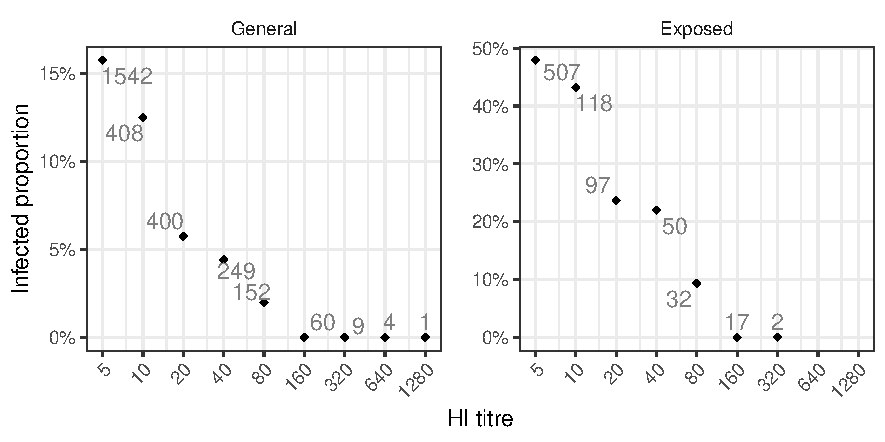
\includegraphics[width=1\textwidth]{../data-plot/hanam-hi-summ-h3n2-light.pdf}
    \caption{
        Ha Nam cohort data for the H3N2 virus from 2009 to 2015. Numbers next to points are the total number of observations in the corresponding group. The left panel shows data for the entire cohort. The right panel shows data from households with at least one infection in a given season. The measurement of 5 corresponds to titres below detectable levels.
    }
    \label{fig:hanam-hi-summ-h3n2}
\end{figure}

\begin{figure}[htp]
    \centering
    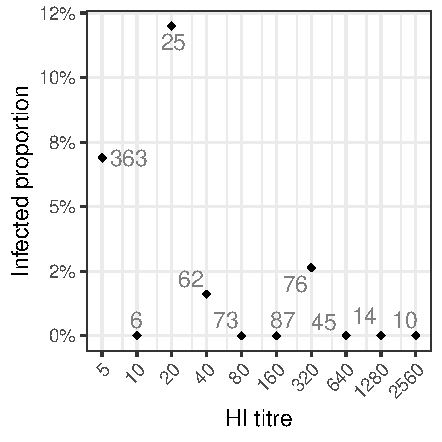
\includegraphics[width=0.5\textwidth]{../data-plot/kiddyvax-main-summ.pdf}
    \caption{
        Kiddivax study data for the B Victoria virus. Numbers next to points are the total number of observations in the corresponding group. The measurement of 5 corresponds to titres below detectable levels.
    }
    \label{fig:kiddivax-main-summ}
\end{figure}
